\documentclass{ximera}

%\usepackage{todonotes}

\newcommand{\todo}{}

\usepackage{esint} % for \oiint
\ifxake%%https://math.meta.stackexchange.com/questions/9973/how-do-you-render-a-closed-surface-double-integral
\renewcommand{\oiint}{{\large\bigcirc}\kern-1.56em\iint}
\fi


\graphicspath{
  {./}
  {ximeraTutorial/}
  {basicPhilosophy/}
  {functionsOfSeveralVariables/}
  {normalVectors/}
  {lagrangeMultipliers/}
  {vectorFields/}
  {greensTheorem/}
  {shapeOfThingsToCome/}
  {dotProducts/}
  {partialDerivativesAndTheGradientVector/}
  {../productAndQuotientRules/exercises/}
  {../normalVectors/exercisesParametricPlots/}
  {../continuityOfFunctionsOfSeveralVariables/exercises/}
  {../partialDerivativesAndTheGradientVector/exercises/}
  {../directionalDerivativeAndChainRule/exercises/}
  {../commonCoordinates/exercisesCylindricalCoordinates/}
  {../commonCoordinates/exercisesSphericalCoordinates/}
  {../greensTheorem/exercisesCurlAndLineIntegrals/}
  {../greensTheorem/exercisesDivergenceAndLineIntegrals/}
  {../shapeOfThingsToCome/exercisesDivergenceTheorem/}
  {../greensTheorem/}
  {../shapeOfThingsToCome/}
  {../separableDifferentialEquations/exercises/}
  {vectorFields/}
}

\newcommand{\mooculus}{\textsf{\textbf{MOOC}\textnormal{\textsf{ULUS}}}}

\usepackage{tkz-euclide}
\usepackage{tikz}
\usepackage{tikz-cd}
\usetikzlibrary{arrows}
\tikzset{>=stealth,commutative diagrams/.cd,
  arrow style=tikz,diagrams={>=stealth}} %% cool arrow head
\tikzset{shorten <>/.style={ shorten >=#1, shorten <=#1 } } %% allows shorter vectors

\usetikzlibrary{backgrounds} %% for boxes around graphs
\usetikzlibrary{shapes,positioning}  %% Clouds and stars
\usetikzlibrary{matrix} %% for matrix
\usepgfplotslibrary{polar} %% for polar plots
\usepgfplotslibrary{fillbetween} %% to shade area between curves in TikZ
%\usetkzobj{all}
\usepackage[makeroom]{cancel} %% for strike outs
%\usepackage{mathtools} %% for pretty underbrace % Breaks Ximera
%\usepackage{multicol}
\usepackage{pgffor} %% required for integral for loops



%% http://tex.stackexchange.com/questions/66490/drawing-a-tikz-arc-specifying-the-center
%% Draws beach ball
\tikzset{pics/carc/.style args={#1:#2:#3}{code={\draw[pic actions] (#1:#3) arc(#1:#2:#3);}}}



\usepackage{array}
\setlength{\extrarowheight}{+.1cm}
\newdimen\digitwidth
\settowidth\digitwidth{9}
\def\divrule#1#2{
\noalign{\moveright#1\digitwidth
\vbox{\hrule width#2\digitwidth}}}




% \newcommand{\RR}{\mathbb R}
% \newcommand{\R}{\mathbb R}
% \newcommand{\N}{\mathbb N}
% \newcommand{\Z}{\mathbb Z}

\newcommand{\sagemath}{\textsf{SageMath}}


%\renewcommand{\d}{\,d\!}
%\renewcommand{\d}{\mathop{}\!d}
%\newcommand{\dd}[2][]{\frac{\d #1}{\d #2}}
%\newcommand{\pp}[2][]{\frac{\partial #1}{\partial #2}}
% \renewcommand{\l}{\ell}
%\newcommand{\ddx}{\frac{d}{\d x}}

% \newcommand{\zeroOverZero}{\ensuremath{\boldsymbol{\tfrac{0}{0}}}}
%\newcommand{\inftyOverInfty}{\ensuremath{\boldsymbol{\tfrac{\infty}{\infty}}}}
%\newcommand{\zeroOverInfty}{\ensuremath{\boldsymbol{\tfrac{0}{\infty}}}}
%\newcommand{\zeroTimesInfty}{\ensuremath{\small\boldsymbol{0\cdot \infty}}}
%\newcommand{\inftyMinusInfty}{\ensuremath{\small\boldsymbol{\infty - \infty}}}
%\newcommand{\oneToInfty}{\ensuremath{\boldsymbol{1^\infty}}}
%\newcommand{\zeroToZero}{\ensuremath{\boldsymbol{0^0}}}
%\newcommand{\inftyToZero}{\ensuremath{\boldsymbol{\infty^0}}}



% \newcommand{\numOverZero}{\ensuremath{\boldsymbol{\tfrac{\#}{0}}}}
% \newcommand{\dfn}{\textbf}
% \newcommand{\unit}{\,\mathrm}
% \newcommand{\unit}{\mathop{}\!\mathrm}
% \newcommand{\eval}[1]{\bigg[ #1 \bigg]}
% \newcommand{\seq}[1]{\left( #1 \right)}
% \renewcommand{\epsilon}{\varepsilon}
% \renewcommand{\phi}{\varphi}


% \renewcommand{\iff}{\Leftrightarrow}

% \DeclareMathOperator{\arccot}{arccot}
% \DeclareMathOperator{\arcsec}{arcsec}
% \DeclareMathOperator{\arccsc}{arccsc}
% \DeclareMathOperator{\si}{Si}
% \DeclareMathOperator{\scal}{scal}
% \DeclareMathOperator{\sign}{sign}


%% \newcommand{\tightoverset}[2]{% for arrow vec
%%   \mathop{#2}\limits^{\vbox to -.5ex{\kern-0.75ex\hbox{$#1$}\vss}}}
% \newcommand{\arrowvec}[1]{{\overset{\rightharpoonup}{#1}}}
% \renewcommand{\vec}[1]{\arrowvec{\mathbf{#1}}}
% \renewcommand{\vec}[1]{{\overset{\boldsymbol{\rightharpoonup}}{\mathbf{#1}}}}

% \newcommand{\point}[1]{\left(#1\right)} %this allows \vector{ to be changed to \vector{ with a quick find and replace
% \newcommand{\pt}[1]{\mathbf{#1}} %this allows \vec{ to be changed to \vec{ with a quick find and replace
% \newcommand{\Lim}[2]{\lim_{\point{#1} \to \point{#2}}} %Bart, I changed this to point since I want to use it.  It runs through both of the exercise and exerciseE files in limits section, which is why it was in each document to start with.

% \DeclareMathOperator{\proj}{\mathbf{proj}}
% \newcommand{\veci}{{\boldsymbol{\hat{\imath}}}}
% \newcommand{\vecj}{{\boldsymbol{\hat{\jmath}}}}
% \newcommand{\veck}{{\boldsymbol{\hat{k}}}}
% \newcommand{\vecl}{\vec{\boldsymbol{\l}}}
% \newcommand{\uvec}[1]{\mathbf{\hat{#1}}}
% \newcommand{\utan}{\mathbf{\hat{t}}}
% \newcommand{\unormal}{\mathbf{\hat{n}}}
% \newcommand{\ubinormal}{\mathbf{\hat{b}}}

% \newcommand{\dotp}{\bullet}
% \newcommand{\cross}{\boldsymbol\times}
% \newcommand{\grad}{\boldsymbol\nabla}
% \newcommand{\divergence}{\grad\dotp}
% \newcommand{\curl}{\grad\cross}
%\DeclareMathOperator{\divergence}{divergence}
%\DeclareMathOperator{\curl}[1]{\grad\cross #1}
% \newcommand{\lto}{\mathop{\longrightarrow\,}\limits}

% \renewcommand{\bar}{\overline}

\colorlet{textColor}{black}
\colorlet{background}{white}
\colorlet{penColor}{blue!50!black} % Color of a curve in a plot
\colorlet{penColor2}{red!50!black}% Color of a curve in a plot
\colorlet{penColor3}{red!50!blue} % Color of a curve in a plot
\colorlet{penColor4}{green!50!black} % Color of a curve in a plot
\colorlet{penColor5}{orange!80!black} % Color of a curve in a plot
\colorlet{penColor6}{yellow!70!black} % Color of a curve in a plot
\colorlet{fill1}{penColor!20} % Color of fill in a plot
\colorlet{fill2}{penColor2!20} % Color of fill in a plot
\colorlet{fillp}{fill1} % Color of positive area
\colorlet{filln}{penColor2!20} % Color of negative area
\colorlet{fill3}{penColor3!20} % Fill
\colorlet{fill4}{penColor4!20} % Fill
\colorlet{fill5}{penColor5!20} % Fill
\colorlet{gridColor}{gray!50} % Color of grid in a plot

\newcommand{\surfaceColor}{violet}
\newcommand{\surfaceColorTwo}{redyellow}
\newcommand{\sliceColor}{greenyellow}




\pgfmathdeclarefunction{gauss}{2}{% gives gaussian
  \pgfmathparse{1/(#2*sqrt(2*pi))*exp(-((x-#1)^2)/(2*#2^2))}%
}


%%%%%%%%%%%%%
%% Vectors
%%%%%%%%%%%%%

%% Simple horiz vectors
\renewcommand{\vector}[1]{\left\langle #1\right\rangle}


%% %% Complex Horiz Vectors with angle brackets
%% \makeatletter
%% \renewcommand{\vector}[2][ , ]{\left\langle%
%%   \def\nextitem{\def\nextitem{#1}}%
%%   \@for \el:=#2\do{\nextitem\el}\right\rangle%
%% }
%% \makeatother

%% %% Vertical Vectors
%% \def\vector#1{\begin{bmatrix}\vecListA#1,,\end{bmatrix}}
%% \def\vecListA#1,{\if,#1,\else #1\cr \expandafter \vecListA \fi}

%%%%%%%%%%%%%
%% End of vectors
%%%%%%%%%%%%%

%\newcommand{\fullwidth}{}
%\newcommand{\normalwidth}{}



%% makes a snazzy t-chart for evaluating functions
%\newenvironment{tchart}{\rowcolors{2}{}{background!90!textColor}\array}{\endarray}

%%This is to help with formatting on future title pages.
\newenvironment{sectionOutcomes}{}{}



%% Flowchart stuff
%\tikzstyle{startstop} = [rectangle, rounded corners, minimum width=3cm, minimum height=1cm,text centered, draw=black]
%\tikzstyle{question} = [rectangle, minimum width=3cm, minimum height=1cm, text centered, draw=black]
%\tikzstyle{decision} = [trapezium, trapezium left angle=70, trapezium right angle=110, minimum width=3cm, minimum height=1cm, text centered, draw=black]
%\tikzstyle{question} = [rectangle, rounded corners, minimum width=3cm, minimum height=1cm,text centered, draw=black]
%\tikzstyle{process} = [rectangle, minimum width=3cm, minimum height=1cm, text centered, draw=black]
%\tikzstyle{decision} = [trapezium, trapezium left angle=70, trapezium right angle=110, minimum width=3cm, minimum height=1cm, text centered, draw=black]


\title{Two Sides}

\begin{document}

\begin{abstract}
one side
\end{abstract}
\maketitle




Tangent lines are tangent to a curve or graph at a tangent point. There must be a point on the curve. At that tangent point, the curve or graph is behaving in some manner, which the tangent line is modeling.  \\

There are two behaviors happening. \\



\textbf{First}, the curve or graph is approaching that point. The graph is connecting up to the point.\\

\textbf{Second}, the tangent lines at approaching points are smoothly turning into the tangent line at the tangent point. \\



There are three situations to consider. \\




\section{Two Sides}


Suppose our tangent point is $(t, f(t))$ and $t$ is inside an open interval in the domain, $t \in (a, b)$. \\


In this situation, we have approaching occurring from both sides and both sides \textbf{must} agree. \\





Here is the graph of the function $f(x) = (x - 3)^2 - 4$.

\begin{image}
\begin{tikzpicture}
     \begin{axis}[
                domain=-10:10, ymax=10, xmax=10, ymin=-6, xmin=-6,
                axis lines =center, xlabel=$x$, ylabel=$y$,
                ytick={-6,-4,-2,2,4,6,8,10},
                xtick={-6,-4,-2,2,4,6,8,10},
                ticklabel style={font=\scriptsize},
                every axis y label/.style={at=(current axis.above origin),anchor=south},
                every axis x label/.style={at=(current axis.right of origin),anchor=west},
                axis on top,
                ]


        \addplot [draw=penColor, very thick, smooth, domain=(0:6),<->] {(x-3)^2 - 4};

        \addplot [color=penColor2,only marks,mark=*] coordinates{(4,-3)};
        


        %\node[penColor] at (axis cs:5,-4) {$(h, k)$};
        %\node[penColor] at (axis cs:5,-9) {$-0.5 x^2 - 5 x + 15.5$};



    \end{axis}
\end{tikzpicture}
\end{image}

A parabola and a point. \\


\textbf{First}, the points on the graph are approaching the point on both sides.  There is no break in the curve. \\


The soon to be tangent point is $(4, 3)$ \\







\begin{image}
\begin{tikzpicture}
     \begin{axis}[
                domain=-10:10, ymax=10, xmax=10, ymin=-6, xmin=-6,
                axis lines =center, xlabel=$x$, ylabel=$y$,
                ytick={-6,-4,-2,2,4,6,8,10},
                xtick={-6,-4,-2,2,4,6,8,10},
                ticklabel style={font=\scriptsize},
                every axis y label/.style={at=(current axis.above origin),anchor=south},
                every axis x label/.style={at=(current axis.right of origin),anchor=west},
                axis on top,
                ]


        \addplot [draw=penColor, very thick, smooth, domain=(0:6),<->] {(x-3)^2 - 4};

        \addplot [color=penColor,only marks,mark=*] coordinates{(4,-3)};
        
        \addplot [draw=penColor2, very thick, smooth, domain=(3:8),<->] {2*(x-4)-3};

        %\node[penColor] at (axis cs:5,-4) {$(h, k)$};
        %\node[penColor] at (axis cs:5,-9) {$-0.5 x^2 - 5 x + 15.5$};



    \end{axis}
\end{tikzpicture}
\end{image}



The tangent line does the best job of modeling the curve right at the tangent point. \\


We know from the derivative or $iRoC_f(x) = 2 (x-3)^2 - 4$, that the slope of this tangent line is $f'(3) = 2 (4-3)^2 = 2$ \\

That gives us a tangent line described by the equation $y = 2 (x - 4) - 3$.











\textbf{Second}, the tangent lines at approaching points smoothly turn into the tangent line at the tangent point...on both sides.





\begin{image}
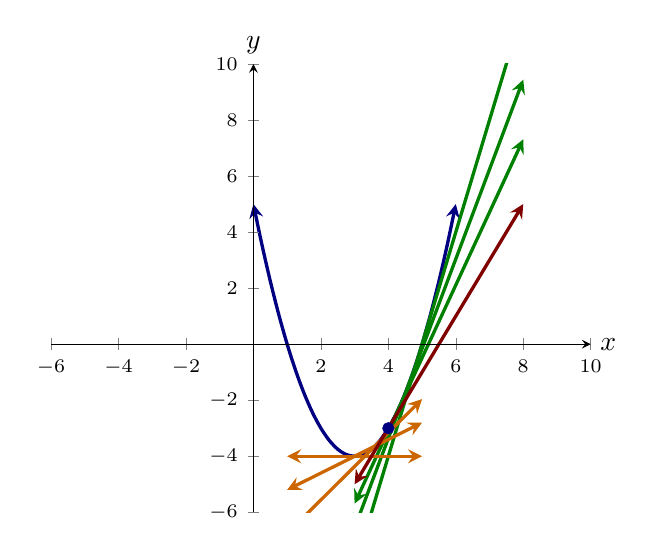
\begin{tikzpicture}
     \begin{axis}[
                domain=-10:10, ymax=10, xmax=10, ymin=-6, xmin=-6,
                axis lines =center, xlabel=$x$, ylabel=$y$,
                ytick={-6,-4,-2,2,4,6,8,10},
                xtick={-6,-4,-2,2,4,6,8,10},
                ticklabel style={font=\scriptsize},
                every axis y label/.style={at=(current axis.above origin),anchor=south},
                every axis x label/.style={at=(current axis.right of origin),anchor=west},
                axis on top,
                ]


        \addplot [draw=penColor, very thick, smooth, domain=(0:6),<->] {(x-3)^2 - 4};

        \addplot [color=penColor,only marks,mark=*] coordinates{(4,-3)};
        
       


        \addplot [draw=penColor4, very thick, smooth, domain=(3:8),<->] {4*(x-5)};
        \addplot [draw=penColor4, very thick, smooth, domain=(3:8),<->] {3.2*(x-4.6)-1.44};
        \addplot [draw=penColor4, very thick, smooth, domain=(3:8),<->] {2.6*(x-4.3)-2.31};

        \addplot [draw=penColor5, very thick, smooth, domain=(1:5),<->] {-4};
        \addplot [draw=penColor5, very thick, smooth, domain=(1:5),<->] {0.6*(x-3.3)-3.82};
        \addplot [draw=penColor5, very thick, smooth, domain=(1:5),<->] {1.2*(x-3.6)-3.64};


          \addplot [draw=penColor2, very thick, smooth, domain=(3:8),<->] {2*(x-4)-3};



        %\node[penColor] at (axis cs:5,-4) {$(h, k)$};
        %\node[penColor] at (axis cs:5,-9) {$-0.5 x^2 - 5 x + 15.5$};



    \end{axis}
\end{tikzpicture}
\end{image}


The tangent lines on the left smootly turn into the tangent line as you move to the right. The tangent lines on the right smootly turn into the tangent line as you move to the left. \\










A function with a discontiuity has a break in the graph.



\begin{image}
\begin{tikzpicture}
     \begin{axis}[
                domain=-10:10, ymax=10, xmax=10, ymin=-6, xmin=-6,
                axis lines =center, xlabel=$x$, ylabel=$y$,
                ytick={-6,-4,-2,2,4,6,8,10},
                xtick={-6,-4,-2,2,4,6,8,10},
                ticklabel style={font=\scriptsize},
                every axis y label/.style={at=(current axis.above origin),anchor=south},
                every axis x label/.style={at=(current axis.right of origin),anchor=west},
                axis on top,
                ]


        \addplot [draw=penColor, very thick, smooth, domain=(0:4),<-] {(x-3)^2 - 4};
        \addplot [draw=penColor, very thick, smooth, domain=(4:6),->] {(x-3)^2 + 1};

        \addplot [color=penColor,only marks,mark=*] coordinates{(4,-3)};
        \addplot [color=penColor,fill=white,only marks,mark=*] coordinates{(4,2)};
        
       



          %\addplot [draw=penColor2, very thick, smooth, domain=(3:8),<->] {2*(x-4)-3};



        %\node[penColor] at (axis cs:5,-4) {$(h, k)$};
        %\node[penColor] at (axis cs:5,-9) {$-0.5 x^2 - 5 x + 15.5$};



    \end{axis}
\end{tikzpicture}
\end{image}













However, if there is a break in the graph, then the two sides might not agree. \\






\begin{image}
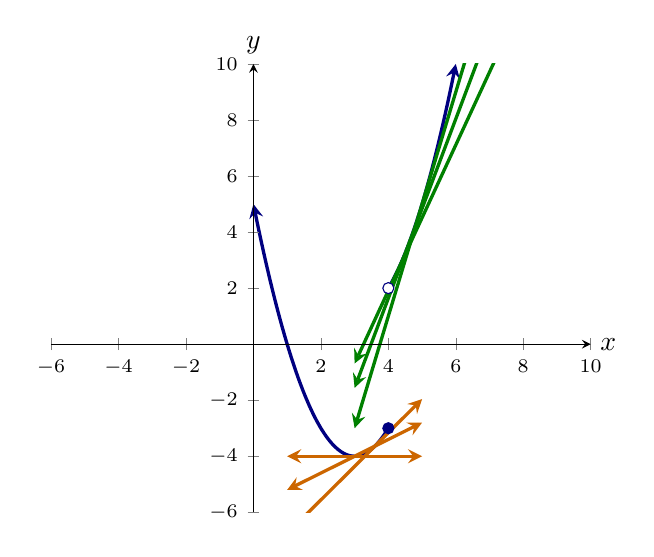
\begin{tikzpicture}
     \begin{axis}[
                domain=-10:10, ymax=10, xmax=10, ymin=-6, xmin=-6,
                axis lines =center, xlabel=$x$, ylabel=$y$,
                ytick={-6,-4,-2,2,4,6,8,10},
                xtick={-6,-4,-2,2,4,6,8,10},
                ticklabel style={font=\scriptsize},
                every axis y label/.style={at=(current axis.above origin),anchor=south},
                every axis x label/.style={at=(current axis.right of origin),anchor=west},
                axis on top,
                ]


        \addplot [draw=penColor, very thick, smooth, domain=(0:4),<-] {(x-3)^2 - 4};
        \addplot [draw=penColor, very thick, smooth, domain=(4:6),->] {(x-3)^2 + 1};

        \addplot [color=penColor,only marks,mark=*] coordinates{(4,-3)};
        \addplot [color=penColor,fill=white,only marks,mark=*] coordinates{(4,2)};
        
       


        \addplot [draw=penColor4, very thick, smooth, domain=(3:8),<->] {4*(x-5)+5};
        \addplot [draw=penColor4, very thick, smooth, domain=(3:8),<->] {3.2*(x-4.6)+3.56};
        \addplot [draw=penColor4, very thick, smooth, domain=(3:8),<->] {2.6*(x-4.3)+2.69};




        \addplot [draw=penColor5, very thick, smooth, domain=(1:5),<->] {-4};
        \addplot [draw=penColor5, very thick, smooth, domain=(1:5),<->] {0.6*(x-3.3)-3.82};
        \addplot [draw=penColor5, very thick, smooth, domain=(1:5),<->] {1.2*(x-3.6)-3.64};


          %\addplot [draw=penColor2, very thick, smooth, domain=(3:8),<->] {2*(x-4)-3};



        %\node[penColor] at (axis cs:5,-4) {$(h, k)$};
        %\node[penColor] at (axis cs:5,-9) {$-0.5 x^2 - 5 x + 15.5$};



    \end{axis}
\end{tikzpicture}
\end{image}

The two sides have tangent lines, but they are not smoothly turning to agree. \\


In this case, we say that there is not tangent line. \\

And, if there is no tangent line, then there is no slope of the tangent line, then the derivative has no value here. \\







So, a derivative implies that there are two sides and the two sides are agreeing. \\



But, there is no need to just throw everything else away.  We can extend our idea of derivative to include just one side. \\ 


































\section{One Side}

Suppose our function has a discontinuity at $t$. \\

Discontiuity means that the number is a domain number and there is a corresponding point on the graph.  The point $(t, f(t))$ is on the graph. \\















\begin{center}
\textbf{\textcolor{green!50!black}{ooooo=-=-=-=-=-=-=-=-=-=-=-=-=ooOoo=-=-=-=-=-=-=-=-=-=-=-=-=ooooo}} \\

more examples can be found by following this link\\ \link[More Examples of Quadratic Behavior]{https://ximera.osu.edu/csccmathematics/precalculus1/precalculus1/quadraticBehavior/examples/exampleList}

\end{center}




\end{document}




